\chapter{\label{chapter:dataflow}Dataflow Scheduling}

A familiar concept from traditional architecture is that of instruction latencies. This is the time it takes an instruction to produce its result. While an integer addition might be able to complete without stalls in the pipeline, a multiply or division most likely will not and will take anywhere from 2 to a few dozen cycles. These latencies, however, are always the same and can be known by the compiler. As a result, the compiler can schedule the instructions as best as possible such that, on an out-of-order pipeline, the pipeline stalls for the least amount of time.

These latencies, however, are still low compared to latencies of a memory read that misses the cache. A read that misses all on-chip caches and needs to read from external memory can take several hundred, or even a thousand cycles. Because the actual latency is so large, varies hugely and depends on run-time conditions, the compiler can often not schedule enough instruction to tolerate the latency. To refer to the these two distinct classes of instructions, we denote the former class of instructions \emph{short-latency} instructions and the latter \emph{long-latency} instructions. Note that long-latency instructions can still complete within a cycle (e.g., a load that hits the L1 cache).

A microgrid core has been designed to use multithreading to hide the latency of long-latency instructions in a single thread. It accomplishes this by flushing the pipeline and switching to another
thread when the pipeline detects that an operand that is required by the current instruction is not available.

\section{Register states}
Since operands are registers, all registers on a microgrid core are extended with state bits that identify whether the register is \emph{full} or \emph{empty}. Normal operations such as integer additions write the register and set the state bits to \emph{full}. Long-latency operations such memory loads set the state bits to \emph{empty} when the operation is issued. When the operation completes, the register is written and its state bits set to \emph{full}. The state transition diagram is shown in figure~\ref{fig:register-states}.

\begin{figure}
 \begin{center}
  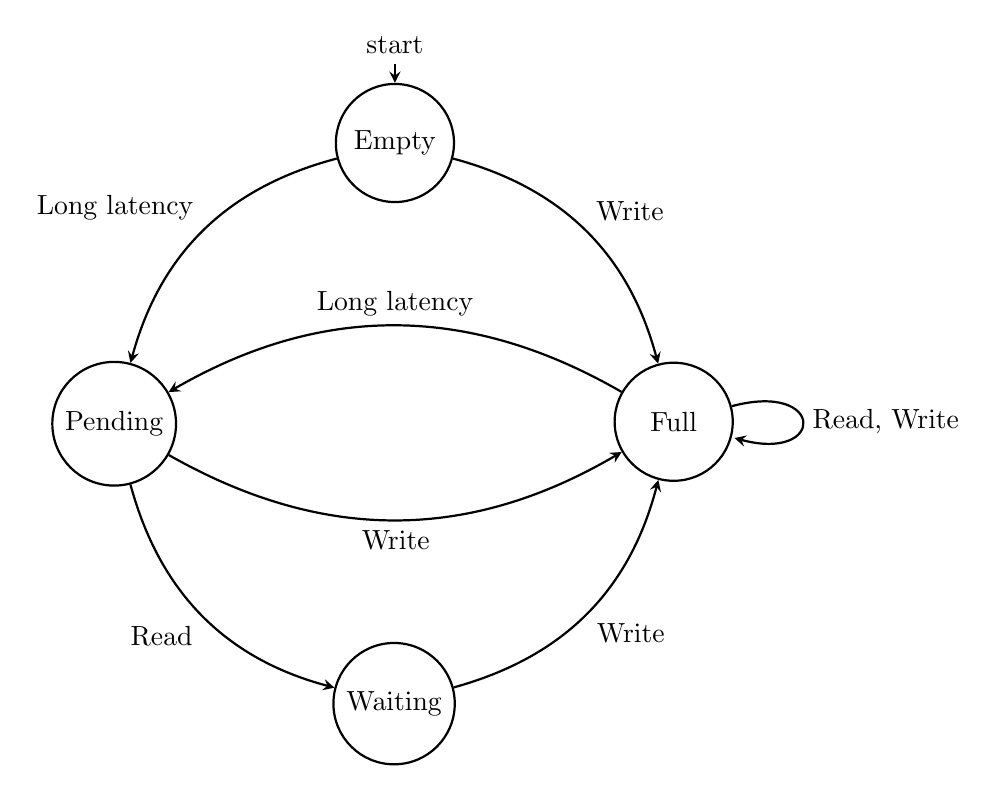
\begin{tikzpicture}[auto,>=stealth,thick,text badly centered]

\begin{scope}[every node/.style={minimum width=1.5cm}]
  \node[draw,circle] (E) {Empty};
  \node[draw,circle,below left=3cm] (P) at (E) {Pending};
  \node[draw,circle,below right=3cm] (W) at (P) {Waiting};
  \node[draw,circle,below right=3cm] (F) at (E) {Full};
\end{scope}
\node[above=1cm] (I) at (E) {start};

\path[->] (I) edge (E)
				  (E) edge [bend right] node [swap] {Long latency} (P)
					(E) edge [bend left]  node        {Write} (F)
		      (P) edge [bend right] node [swap] {Read} (W)
		      (W) edge [bend right] node [swap] {Write} (F)
			    (F) edge [bend right] node [swap] {Long latency} (P)
			    (P) edge [bend right] node [swap] {Write} (F)
			    (F) edge [loop right] node        {Read, Write} (F);

\end{tikzpicture}
  \caption{Register state transitions.}
  \label{fig:register-states}
 \end{center}
\end{figure}

\section{\label{sec:control-stream}Thread control stream}
As described above, if the pipeline executes an instruction that does not have its operands available, the pipeline (before the offending instruction) is flushed of the thread's instructions and execution is switched to another thread. This flush creates several bubbles in the pipeline for every missed data dependency. The number of bubbles depends on the number of stages between the start of the pipeline and the place where the registers have been read and the decision is made to flush or not based on their state. In a traditional 6-stage pipeline, this can be around 3 cycles. To avoid this cost, a secondary instruction stream is read by the pipeline. This secondary stream consists of two bits per instruction, indicating one of several thread control operations to perform after reading it:

\begin{itemize}
\item Do nothing; continue executing from this thread as normal.
\item Switch thread; if another thread is available for execution, switch to it after fetching this instruction.
\item End thread; after fetching this instruction, end the thread. Note that this implies a switch.
\end{itemize}

Having the first two options available, the compiler can 'tag' instructions with the \emph{switch} value in the secondary instruction stream (also called the \emph{control stream}). With this, the compiler tells the hardware that this instruction uses, or can use, the result of a long-latency operation. The pipeline, upon seeing the \emph{switch} bit set after fetching the instruction, will immediately switch to another thread without waiting to see if the operands are available or not. This way, the pipeline before the instruction does not contain intruction from the current thread and the flush does not create bubbles.

The control stream is interleaved with the instruction stream. Since each control instruction is 2 bits wide, on a typical 32-bit RISC architecture, a single instruction word can contain 16 control instructions, enough to match 16 regular instructions. 16 32-bit instructions fit exactly in a 64-bit cache-line. Thus, if we sacrifice the first regular instruction and store a \emph{control word} containing 16 control words in its place, we can store 15 instructions and their control instructions in a single 64-byte cache-line. This is illustrated in figure~\ref{fig:control-word}. Having both streams in a single cache-line ensure that only a single cache-line has to be loaded for a thread, no matter its program counter. Note that this means that the size of an I-cache line must be at least the size of the instructions covered by a single control word. In the example above, a 32-byte I-Cache line can be created by only using half of the control word (thus covering only 7 instructions).

The cost of this optimization is additional logic in the assembler and hardware to recognize that the first instruction in any cache-line is a special control word that should not be executed. This matters, for instance, with labels, branches or return-from-procedure. If the target is the beginning of a cache-line, the label or PC must be updated to point to the instruction after the control word.

\begin{figure}
 \begin{center}
  \begin{tikzpicture}[auto,>=stealth,thick,text badly centered]

\begin{scope}[start chain, node distance=0cm,every node/.style={draw,rectangle,outer sep=0cm,minimum width=8em,minimum height=2em}]]
  \node[on chain] (CW) {Control Word};
  \node[on chain] (I1) {Instr$_1$};
  \node[on chain] (I2) {Instr$_2$};
  \node[on chain] (I3) {\ldots};
  \node[on chain] (I15) {Instr$_{15}$};
\end{scope}

\node[above] (B0) at (CW.north west) {0};
\node[above] at (CW.north east) {32};
\node[above] at (I1.north east) {64};
\node[above] at (I2.north east) {96};
\node[above] at (I3.north east) {480};
\node[above] at (I15.north east) {512};

\node[left] at (B0.west) {bytes};

\begin{scope}[start chain, node distance=0cm,every node/.style={draw,rectangle,outer sep=0cm,minimum width=8em,minimum height=2em}]]
  \node[on chain,above=2cm,anchor=south west] (C0) at (CW.north west) {CI$_0$};
  \node[on chain] (C1) {CI$_1$};
  \node[on chain] (C2) {CI$_2$};
  \node[on chain] (C3) {\ldots};
  \node[on chain] (C15) {CI$_{15}$};
\end{scope}

\node[above] (b0) at (C0.north west) {0};
\node[above] at (C0.north east) {2};
\node[above] at (C1.north east) {4};
\node[above] at (C2.north east) {6};
\node[above] at (C3.north east) {30};
\node[above] at (C15.north east) {32};

\node[left] at (b0.west) {bits};

\begin{scope}[dashed]
  \draw (CW.north west) -- (C0.south west);
  \draw (CW.north east) -- (C15.south east);
\end{scope}

\end{tikzpicture}
  \caption{Cache line with control word. Shown is the control word on an architecture with 32-bit instructions and a 512-bit cache-line. Control Instruction CI$_i$ is associated with instruction Instr$_i$. CI$_0$ is associated with the control word itself and is unused.}
  \label{fig:control-word}
 \end{center}
\end{figure}

\paragraph{Alternatives}

As an alternative, the ``end thread'' control instruction can also be implemented as a normal instruction to bring the number of bits per instructions in the control stream down to 1. The advantage of this approach would be that a single control word can now cover twice the number of instructions. This means that a single I-cache line can be twice the size. On a machine with 32-bit instructions, this is 128 bytes instead of 64 bytes. The disadvantage is that very small threads that operate on arrays (i.e., array addition) will grow by one instruction, which is a significant amount on those levels of granularity. In the current design, 128-byte cache-line were deemed too big for general purpose as this point in time, so ``sacrificing'' them for not having the downside mentioned above seemed a sane path.

Another alternative is to switch on every cycle (interleaved multi-threading) and remove the \emph{switch} control instruction. This, again, has the benefit of enabling larger I-cache lines. However, the cost of this is two-fold. First, every time a thread switch occurs, the family table and thread table must be read for the chosen thread's information that's required in the pipeline. At the end of the pipeline, additional logic required for switching out the old thread also requires accesses to the thread table and thread queues. This actions cost energy, which can be avoided since the compiler can statically determine if a switch is unnecessary. Secondly, when a thread switch occurs, the old thread (assuming it does not suspend) cannot be re-executed by the pipeline until several cycles later. The thread needs to first traverse the pipeline and then one or two thread queues before it is available to the pipeline again. If there are not enough threads to tolerate this rescheduling latency, the pipeline will have to execute nops until a thread becomes available. In the worst case, only two threads are available. Given a six-stage pipeline and two thread queues, the reschedule latency is 8 cycles, meaning performance is now 25\% of what it could have been had the pipeline not switched blindly on every cycle.

